\documentclass[pdf, handout]{beamer}
\mode<presentation>{\usetheme{boxes}}
%% preamble
 \setbeamertemplate{headline}{}
\setbeamertemplate{section page}[mine]
\title{An introduction to Principal Component Analysis}
\subtitle{}
\author{Ramon van den Akker (Tilburg University)}
\date{}
%%
\usepackage{array}
\usepackage{multirow}

\newcommand\MyBox[2]{
  \fbox{\lower0.75cm
    \vbox to 1.7cm{\vfil
      \hbox to 1.7cm{\hfil\parbox{1.4cm}{#1\\#2}\hfil}
      \vfil}%
  }%
}

%%
\usepackage{algorithm}
\usepackage{algorithmic}
\usepackage{amsmath}
\usepackage{graphics}
\usepackage{multicol}
\usepackage{color}
\usepackage{hyperref}
\definecolor{webbrown}{rgb}{.6,0,0}
\definecolor{webgreen}{rgb}{0,.5,0}
\usepackage{subfigure}
\usepackage{graphicx}
%\usepackage{pstricks,pst-grad}
%\renewcommand{\E}{\operatorname{E}}
\newcommand{\distr}{\sim}
\newcommand{\var}{\operatorname{var}}
\newcommand{\argmin}{\mathop{\mathrm{arg\,min}}}
\newcommand{\rank}{\operatorname{rank}}
\newcommand{\calF}{\mathcal{F}}
\newcommand{\calI}{\mathcal{I}}
\newcommand{\SR}{\mathbb{R}}
\newcommand{\rN}{\mathrm{N}}
\newcommand{\rd}{\mathrm{d}}
\newcommand{\e}{\operatorname{e}}
\newcommand{\Bin}{\operatorname{Bin}}
\newcommand{\kbin}{\operatorname{b}}
\newcommand{\lin}{\operatorname{lin}}
\newcommand{\kansq}{\mathbb{Q}}
\newcommand{\rH}{\mathrm{H}}
%\newarrow{hulp}{<}{filler}{middle}{filler}{head}
\DeclareMathOperator*\ster{*} \DeclareMathOperator*\argmax{argmax}
\usepackage{color}
\newtheorem{Def}{Definition}
\newtheorem{Ass}{Assumption}
\newtheorem{Concl}{Conclusion}
\newcommand{\cov}{\operatorname{cov}}
%%

\AtBeginSection{\frame{\sectionpage}}
%\AtBeginSubsection{\frame{\subsectionpage}}
\newtranslation[to=greek]{Section}{En'othta}
\newtranslation[to=greek]{Subsection}{Upoen'othta}

\defbeamertemplate{section page}{mine}[1][]{%
  \begin{centering}
    {\usebeamerfont{section name}\usebeamercolor[fg]{section name}#1}
    \vskip1em\par
    \begin{beamercolorbox}[sep=12pt,center]{part title}
      \usebeamerfont{section title}\insertsection\par
    \end{beamercolorbox}
  \end{centering}
}

\defbeamertemplate{subsection page}{mine}[1][]{%
  \begin{centering}
    {\usebeamerfont{subsection name}\usebeamercolor[fg]{subsection name}#1}
    \vskip1em\par
    \begin{beamercolorbox}[sep=8pt,center,#1]{part title}
      \usebeamerfont{subsection title}\insertsubsection\par
    \end{beamercolorbox}
  \end{centering}
}

%%
\begin{document}
% title frame
\begin{frame}
\titlepage
\end{frame}

\begin{frame}{Agenda}
\tableofcontents
\end{frame}

%
\section{Introduction and outline PCA}

\begin{frame}{Dimension reduction}
\begin{center}
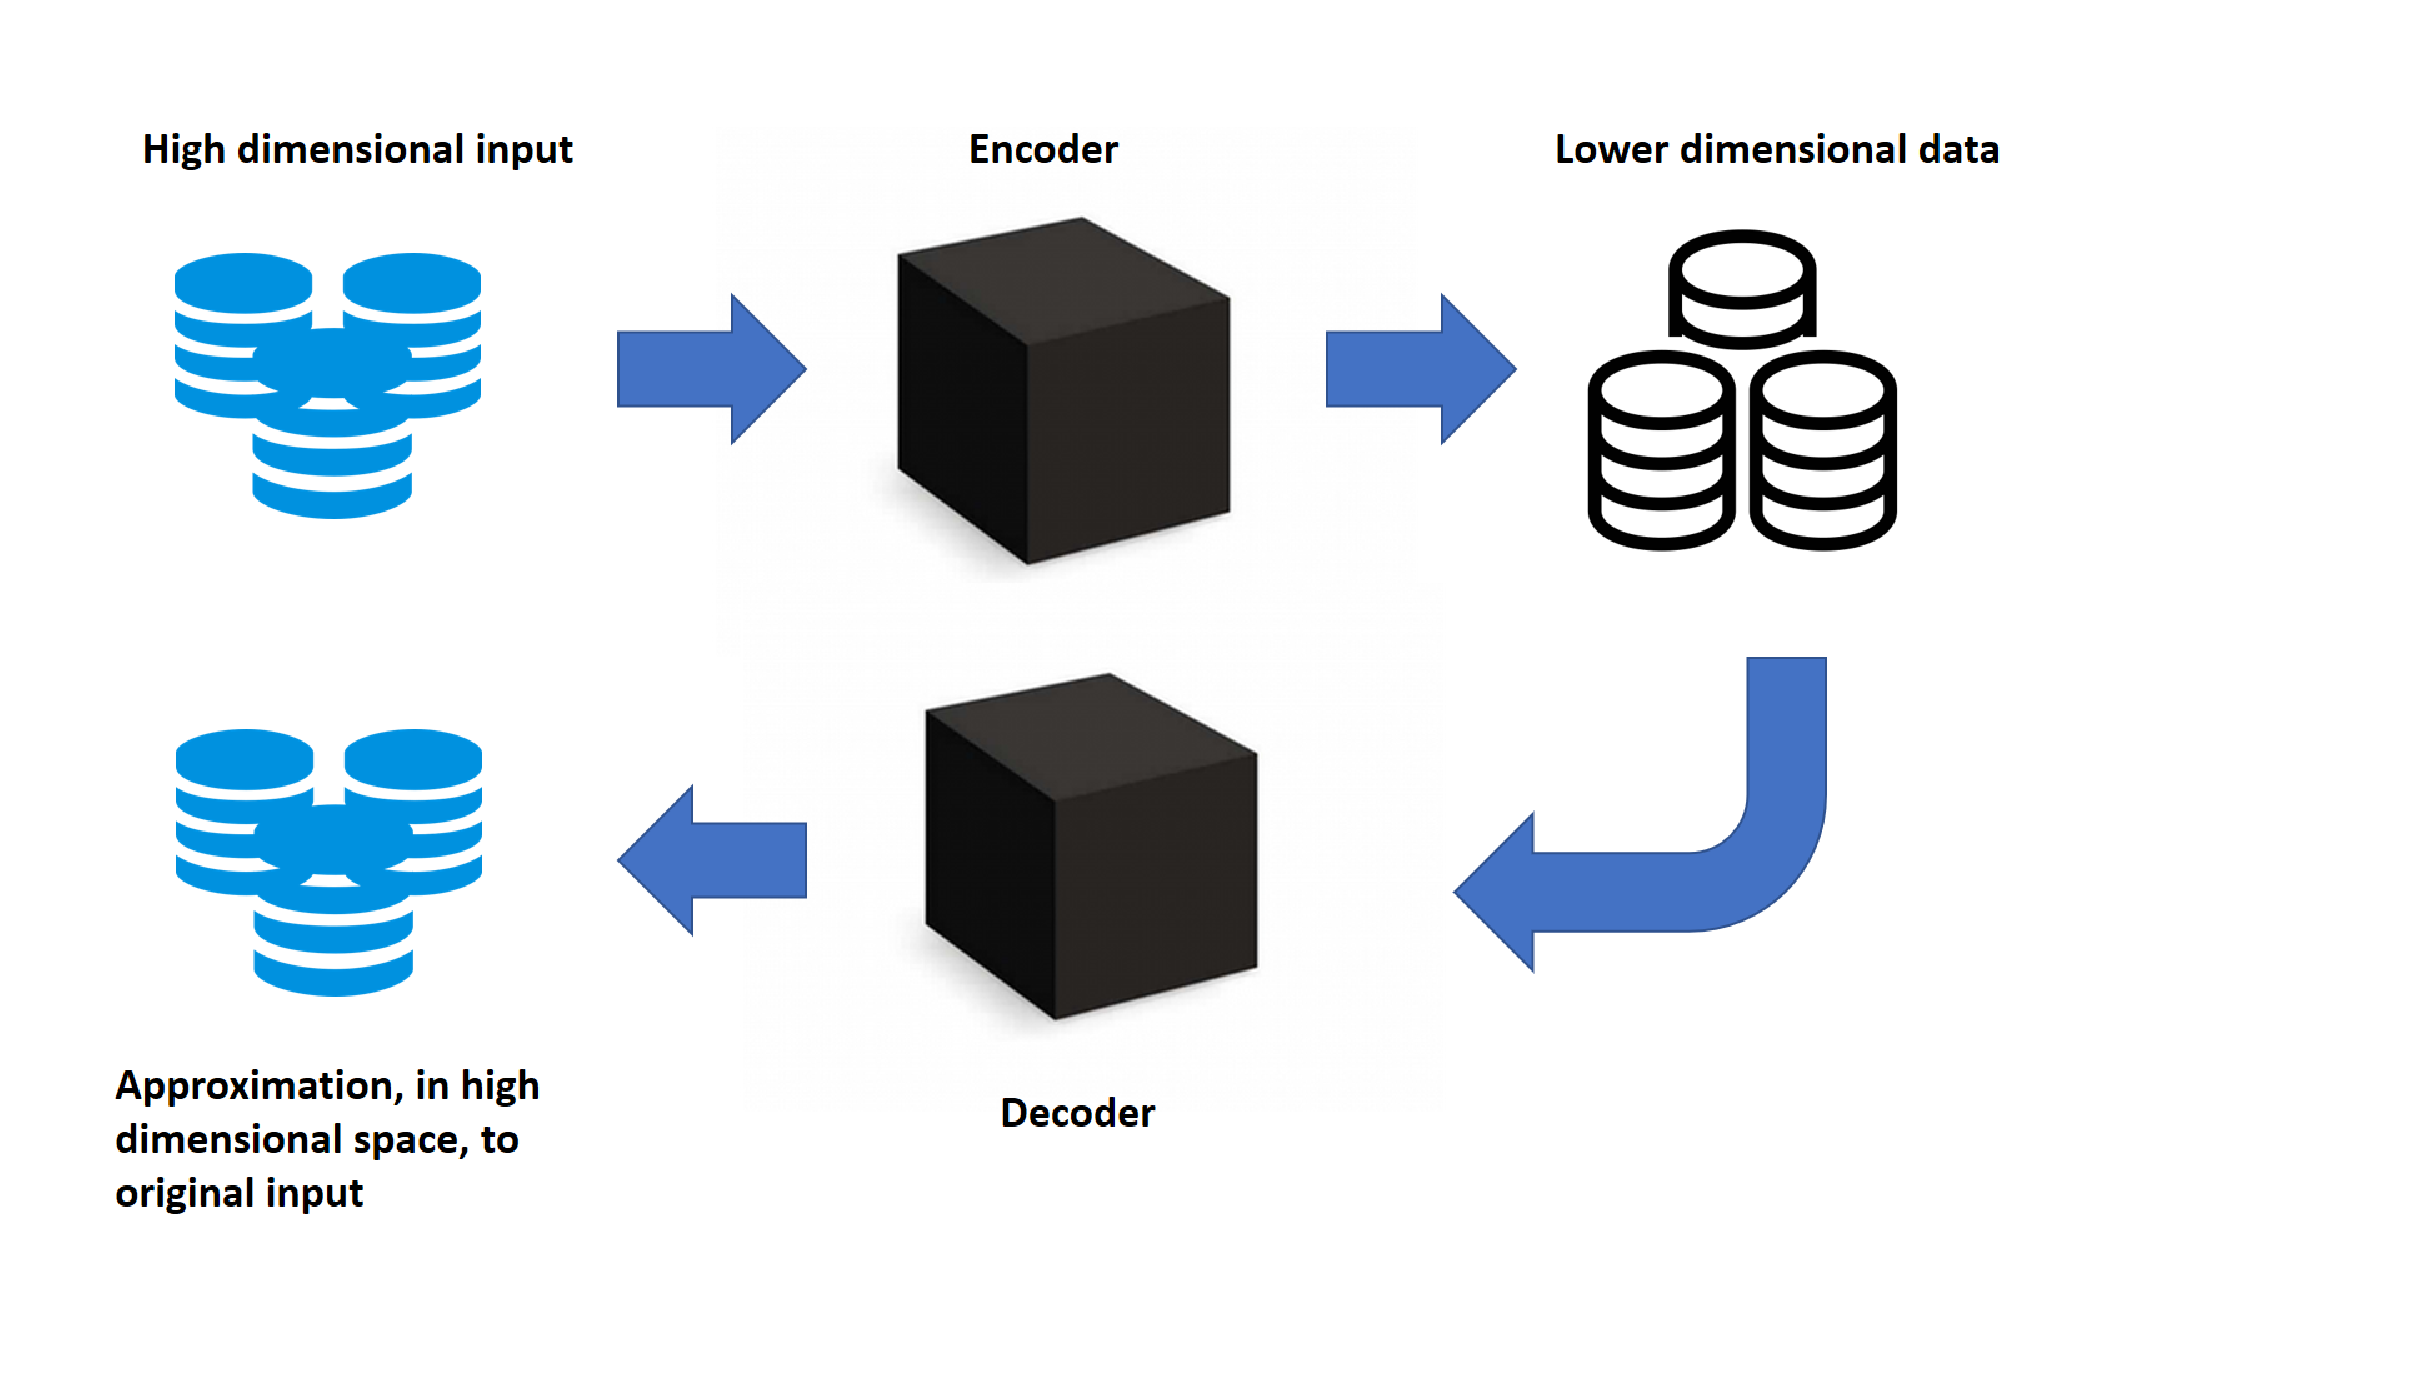
\includegraphics[width=0.8\textwidth]{plaatje_autoencoder}
\end{center}
\textbf{Applications:}
\begin{itemize}
\item data compression 
\item  reduction dimension features  
\item noise removal
\item visualisation
\item anomaly detection
\end{itemize}
\end{frame}



\begin{frame}{Agenda}
\begin{itemize}
\item we discuss Principal Component Analysis (PCA)
\begin{itemize}
\item dates back to  Pearson  (1901) and Hotelling (1933)
\end{itemize}
\item see, for example, Van der Maaten et al. (2009) for review of dimension reduction techniques
\end{itemize}
\end{frame}


\begin{frame}{Outline - PCA}
\textbf{Heuristic description:} \\
\begin{itemize}
\item encoding: find `small' number of directions in input space that explain variation in data as well as possible
\item decoding: represent data in original dimension by projecting along those directions
\end{itemize}
\end{frame}

\begin{frame}{Outline - PCA}
\vspace{-.1cm}
\textbf{Training:}
\begin{itemize}
\item given $p$-dimensional observations $X_1,\dots,X_n$ with mean $\mu=\mathbb{E}X_i$
\item choice for dimension encoder is made ($d< \min\{p, n\}$)
\item $p$-dimensional vectors $w_1,\dots,w_d$,  are constructed (\emph{principal components}) and stored
\end{itemize}
\textbf{Encoding of observations:} \\
For  $p$-dimensional observation $x$ (can also be new observation):
\begin{itemize}
\item calculate \emph{principal scores}  $s_1 = w_1^\prime (x-\hat\mu),\dots, s_d=w_d^\prime (x-\hat\mu)$
\item store $d$-dimensional $(s_1,\dots,s_d)$ and throw $x$ itself away
\end{itemize}
\textbf{Decoding of observations:} \\
Approximation of $x$ in $\mathbb{R}^p$  by:
\[
x_d  = \mu + \sum_{j=1}^d s_j w_j  \in\mathbb{R}^p
\]
\vspace{.25cm}
Need to store $d\times p + \color{blue}{n\times d}$ numbers instead of 
$\color{red}{n\times p}$.
\end{frame}






\begin{frame}{Intuition}
``Best'' reduction to dimension 1 of 2-dimensional data?
\begin{center}
\includegraphics[width=0.8\textwidth]{pca-eps-converted-to}
\end{center}
Such `directions' in data are described by covariance matrix data 
\end{frame}




\begin{frame}{Intuition}
Approximate observation $\tilde x$ by  $s \tilde x \in\mathbb{R}^2$, where $s=\tilde x^\prime u_1$:
\begin{center}
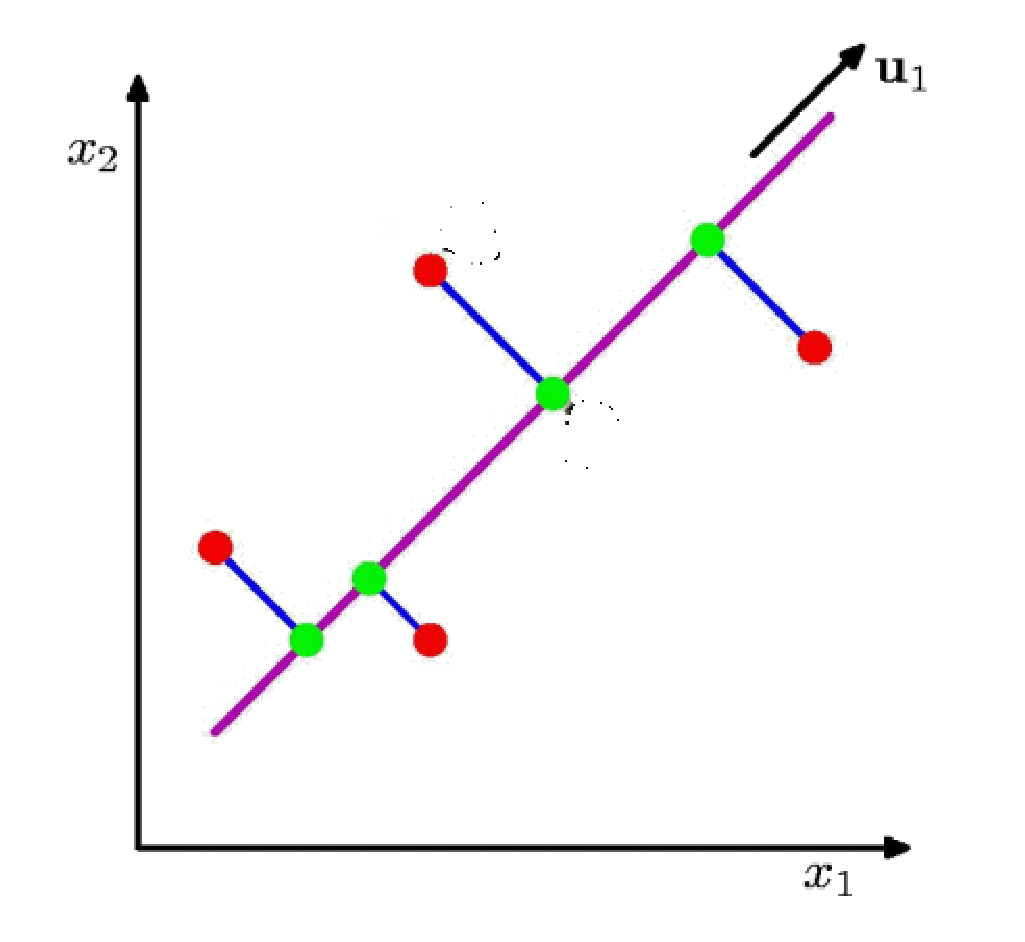
\includegraphics[width=0.8\textwidth]{pca2}
\end{center}


\end{frame}


\begin{frame}{Setup}
\textbf{Setup:} \\
Consider $p$-dimensional random vector $X$ with mean $0_p$ and \emph{known} $p\times p$ positive definite covariance matrix 
$\Sigma$
\begin{itemize}
\item later on we will consider situation in which $\Sigma$ is unknown and have i.i.d. observations $X_1,\dots,X_n$ available
\end{itemize}
\vspace{.5cm}
\textbf{Goal:} \\
Construct, for $d=1,\dots,p-1$, linear subspace of dimension $d$ that explains "as much as possible variation" in $X$ 
\\
\vspace{.5cm}
\textbf{Remarks:} 
\begin{itemize}
\item \textbf{First we will consider $\mu=0$ and $\Sigma$ to be known}. Afterwards, we will
discuss how to proceed in case $\mu\neq 0$ and $\Sigma$ are unknown.
\end{itemize}
\end{frame}

\section{PCA - derivation}


\begin{frame}{PCA - derivation}
We will exploit \textbf{spectral theorem:} \\
As $\Sigma$ is real, symmetric and positive definite matrix we have:
\begin{itemize}
\item there are $p$ real, positive eigenvalues  $\lambda_1\geq \lambda_2 \geq \dots\geq \lambda_p> 0$ and corresponding (real) eigenvectors 
$u_1,\dots, u_p\in\mathbb{R}^p$ with
\begin{itemize}
\item $\|u_j\|^2 = u_j^\prime u_j =1$
\item $u_j^\prime u_i =0$ for $i\neq j$, i.e. eigenvectors are orthogonal
\end{itemize}  
\item $\Sigma$ can be written as:
\[
\Sigma = U \Lambda U^\prime = \sum_{j=1}^p \lambda_j u_j u_j^\prime
\]
where $\Lambda =\operatorname{diag}(\lambda_1,\dots,\lambda_p)$ and
$U=[ u_1 \,\, \cdots \,\, u_p]$
\item $U$ is orthogonal: 
\begin{itemize}
\item $U^\prime U=U U^\prime = I_p$ 
\item $U^{-1}=U^\prime$
\end{itemize}
\item the eigenvectors $u_j$ are called \emph{principal components}
\end{itemize}
\end{frame}




\begin{frame}{PCA - derivation}
Spectral decomposition yields (please note that $X$ is random vector)
\[
\color{blue} X = I_p X = \color{black}(U U^\prime) X=U (U^\prime X) =  \color{blue}  \sum_{j=1}^p  (X^\prime u_j)  u_j.
\]
Note that this represents $X$ in the coordinate system determined by the eigenvectors $u_1,\dots,u_p$. Approximate $X$ by
\[
X_{d} = \sum_{j=1}^{\color{blue} d \color{black}}  (X^\prime u_j)  u_j.
\]
We have
\begin{align*}
\operatorname{var}   (X^\prime u_j)  
&=  u_j^\prime \operatorname{var}(X)  u_j = u_j^\prime U\Lambda U^\prime u_j 
= \lambda_j.  
\end{align*}
And, for $k\neq j$,
\begin{align*}
\operatorname{cov}\left( X^\prime u_j, X^\prime u_k\right)  
&=  u_j^\prime \operatorname{var}(X)  u_k = u_j^\prime U\Lambda U^\prime u_k 
= 0. 
\end{align*}
\end{frame}

\begin{frame}{PCA - derivation}
For approximation error, $\varepsilon_d=X-X_d$, we obtain
\begin{align*}
\color{blue}\mathbb{E}\|\varepsilon_d\|^2&=\color{black}
 \mathbb{E} \left\| \sum_{j=d+1}^p (X^\prime u_j)  u_j \right\|^2 = 
\sum_{j=d+1}^p \mathbb{E}   (X^\prime u_j)^2
=\color{blue} \sum_{j=d+1}^p \lambda_j.  
\end{align*}
And, similarly,
\begin{align*}
\mathbb{E} \| X \|^2    &=  \sum_{j=1}^p \lambda_j \text{ and }
\mathbb{E} \| X_{d} \|^2 =  \sum_{j=1}^d \lambda_j.
\end{align*}
Measure for variation captured by first $d$ principal components:
\[
\frac{\sum_{j=1}^d \lambda_j  }{  \sum_{j=1}^p \lambda_j } \left( \times 100 \% \right) 
\]
\end{frame}

\begin{frame}{PCA}
\begin{itemize}
\item $p$-dimensional vectors $w_1=u_1,\dots,w_d=u_d$ are called the first $d$ \emph{principal components}
\item dimension reduction by using first $d$ principal components:
\begin{itemize}
\item replace $p$-dimensional
observation $\mathbf{x}$ by \emph{principal scores} 
\[
s_j=w_j^\prime (\mathbf{x} - \mu)\in\mathbb{R}, \quad j=1,\dots,d 
\] 
\end{itemize}
\item approximation/reconstruction of $\mathbf{x}$ by
\[
x_{PCA} =\mu + \sum_{j=1}^d s_j w_j    \in \mathbb{R}^p
\]
\item applying PCA to observations $\mathbf{x}_1,\dots,\mathbf{x}_n$: instead of storing $np$ numbers, we need to store $p+dp + nd$ numbers
\end{itemize}
\end{frame}



\section{PCA - standard derivation}


\begin{frame}{PCA - alternative derivation}
\textbf{Procedure} (with $d\leq p$):
\begin{itemize}
\item determine $w_1^\prime X$ with $\| w_1 \|=1$ such that $\var ( w_1^\prime X)$ is maximal
\pause\item determine $w_2^\prime X$ with $\| w_2 \|=1$  and $\cov( w_1^\prime X, w_2^\prime X ) =0$
such that $\var ( w_2^\prime X)$ is maximal
\item[] $\vdots$
\pause
\item determine $w_d^\prime X$ with $\| w_d \|=1$  and $\cov( w_j^\prime X, w_d^\prime X) =0$ for $j=1,\dots,d-1$
such that $\var ( w_d^\prime X)$ is maximal
\end{itemize}
\end{frame}

\begin{frame}{PCA - alternative derivation}
\vspace{-.25cm}
First principal component $w_1$ solves:
\[
\max_{\alpha \in\mathbb{R}^p :\, \| \alpha \|=1 } \var ( \alpha^\prime X) = \alpha^\prime \Sigma \alpha
\]
\pause
Use method of Lagrange mulipliers:
\[
\max_{\alpha \in\mathbb{R} ,\, \lambda\in\mathbb{R}} \mathcal{L}(\alpha,\lambda)= \max_{\alpha \in\mathbb{R} ,\, \lambda\in\mathbb{R}} \alpha^\prime \Sigma \alpha - \lambda (   \alpha^\prime \alpha -1)
\]
Stationary point follows from solving:
\begin{align*}
0&=\frac{\rd}{\rd \alpha} \mathcal{L}(\alpha,\lambda) = 2\Sigma \alpha - 2 \lambda \alpha \\
1&=\alpha^\prime \alpha
\end{align*}
which yields
\color{blue} $\Sigma\alpha =\lambda \alpha$ \color{black}
i.e. $\alpha$ is eigenvector of $\Sigma$ corresponding to eigenvalue $\lambda$
\end{frame}




\begin{frame}{PCA - alternative derivation}
From F.O.C. we obtained:
\[
\Sigma \alpha =\lambda \alpha
\]
As we want to maximize, use constraint $\|\alpha\|=1$,
\[
\alpha^\prime \Sigma \alpha = \alpha^\prime (\Sigma \alpha )
=\alpha^\prime \lambda \alpha = \lambda
\]
it follows that \color{blue} $w_1=u_1 $ \color{black} and \color{blue} $\lambda=\lambda_1$
\end{frame}

\begin{frame}{PCA - alternative derivation}
\begin{itemize}
\item suppose we have already shown $w_j=u_j$ for $j=1,\dots,d-1$
\end{itemize}
Note that
\begin{align*}
\color{blue} 0=\color{black}\cov( w_j^\prime X, w_d^\prime X)=w_d^\prime \Sigma w_j=
\color{blue} \lambda_j w_d^\prime w_j \text{ for } j=1,\dots,d-1
\end{align*}
To determine $w_d$ we need to solve:
\[
\max_{\substack{ \alpha \in\mathbb{R}^p :\, \| \alpha \|=1 \\ 
\cov(w_d^\prime X, w_j^\prime X)=0,\,\, j=1,\dots,d-1 }} \var ( \alpha^\prime X) = \alpha^\prime \Sigma \alpha
\]
\end{frame}

\begin{frame}{PCA - alternative derivation}
Use method of Lagrange mulipliers:
\[
\max_{\substack{\alpha \in\mathbb{R}^p \\ \lambda\in\mathbb{R},\kappa\in\mathbb{R}^{d-1}}}  \alpha^\prime \Sigma \alpha - \lambda (   \alpha^\prime \alpha -1)
-2\sum_{j=1}^{d-1} \kappa_j ( w_j^\prime \Sigma\alpha -0)
\]
Stationary point follows from solving:
\begin{align*}
0&=\frac{\rd}{\rd \alpha} \mathcal{L}(\alpha,\lambda) = 2\Sigma \alpha -  2\lambda \alpha- 2\sum_{j=1}^{d-1}\kappa_j \Sigma w_j \\
1&=\alpha^\prime \alpha \\
0&=\alpha^\prime\Sigma  w_j \text{ for } j=1,\dots,d-1
\end{align*}
\end{frame}

\begin{frame}{PCA - alternative derivation}
Multiplying first equation by $w_j$, with $j\in\{1,\dots,d-1\}$, yields
\[
w_j^\prime \Sigma \alpha =\lambda w_j^\prime \alpha + \sum_{j=1}^{d-1} \kappa_j \lambda_j 
\]
Inserting $0=w_j^\prime \Sigma \alpha =  \lambda_j \alpha^\prime w_j =0$ we obtain \color{blue} $\kappa_j=0$.
\color{black} Hence
\[
\Sigma \alpha = \lambda\alpha
\]
As eigenvectors $u_1,\dots,u_{d-1}$ cannot be used: $w_d = u_d$, the eigenvector corresponding to eigenvalue $\lambda_d$
\end{frame}


\section{Implementation and remarks}

\begin{frame}{Implementation}
\begin{itemize}
\item we have an algorithm for the case $\mu=0$ and $\Sigma$ is known
\item now consider situation in which $\Sigma$, of rank $p$, is unknown and $\mu=\mathbb{E}X\neq 0_p$,  but have i.i.d. observations $Y_1,\dots,Y_n$ available 
\item just use `anology principle': 
\begin{itemize}
\item estimate $\Sigma$ by sample covariance matrix
\[
\hat \Sigma = \frac{1}{n-1} \sum_{i=1}^n (Y_i - \hat{\mu})(Y_i - \hat{\mu})^\prime 
\]
with $\hat{\mu}=n^{-1}\sum_{i=1}^n Y_i$
\item apply PCA using $\hat\Sigma$ and centered observations
$X_i = Y_i - \hat{\mu}$.
\item rank of $\hat\Sigma$ is at most $n-1$
\item if $n>p$ (and true $\Sigma$ has full column rank) then you we will typically have $\operatorname{rank}(\hat\Sigma)=p$
\item if $\hat\Sigma$ is not of rank $p$, then $d=\operatorname{rank(\hat\Sigma)}$ is the maximal number of
principal components you can use
\end{itemize}
\begin{itemize}
\item estimators  $\hat w_1,\dots,\hat w_d$ of of principal components $w_1,\dots,w_d$
\end{itemize}
\end{itemize}
\end{frame}

\begin{frame}{Implementation - to scale or not to scale?}
\begin{itemize}
\item from the theory it is clear that PCA is not scale invariant (see notebook for numerical illustration), so the results depend on the scale of the variables
\begin{itemize}
\item for example, using `expenditures in euro' can yield different results
compared to using `expenditures in cents'
\end{itemize}
\item often variables are scaled by their (estimated) standard deviation before
applying PCA
\item not always a good idea to preprocess variables: 
if variables have been measured in same units
\end{itemize}
\end{frame}
%
\begin{frame}{Remarks - Statistical Properties}
Statistical properties?
\begin{itemize}
\item not trivial
\item consistency and asymptotic normality (for principal components) have been studied for various settings:
\begin{itemize}
\item $p$ is fixed and $n\to\infty$ 
\item $n$ fixed and $p\to\infty$ (useful for ``high-dimensional, but small data'')
\item both $p\to\infty$
and $n\to\infty$ (sometimes with restrictions on relative speed, like $n/d\to c\in(0,\infty)$) 
\item references:  Anderson, T.W. (1963), Jung et al. (2009), and
Shen et al. (2016)
\end{itemize}
\end{itemize}
\end{frame}


\begin{frame}{Remarks - selected actuarial applications}
\begin{itemize}
\item use of PCA in yield curve modelling
\begin{itemize}
\item see, for example, Diebold and Li (2006), Barber and Copper (2012)
\end{itemize}
\item use in mortality and longevity modelling
\begin{itemize}
\item see, for example, Yanga et al. (2010)
\end{itemize}
\item use in car insurance
\begin{itemize}
\item see, for example, Segovia-Gonzalez (2009) and
Zhu and W\"{u}thrich (2020)
\end{itemize}
\end{itemize}
\end{frame}


\section{Demo}

\begin{frame}{Demo}
See notebook
\end{frame}


\section{References}


\begin{frame}{References}
\tiny
\begin{itemize}
\item Anderson, T.W. (1963). 
Asymptotic Theory for Principal Component Analysis.
\emph{The Annals of Mathematical Statistics} 34, pp.122-148.
\item Barber, J.R. and M.L. Copper (2012).
Principal component analysis of yield
curve movements. \emph{Journal of Economics and Finance} 36, pp.750--765.
\item Diebold, F.X. and C. Li (2006). 
Forecasting the term structure of government
bond yields. \emph{Journal of Econometrics} 130, pp.337--364.
\item 
Jung, S. and J. S. Marron (2009). PCA consistency in high dimension low sample
size context. \emph{The Annals of Statistics} 37, pp.4104--4130.
\item Shen, D. H. Shen, and J.S. Marron (2016). \emph{Journal of Machine Learning Research} 17, pp.1-34
\item van der Maaten, L.J.P., E.O. Postma, and H.J. van den Herik. Dimensionality Reduction: A Comparative Review. Tilburg University Technical Report, TiCC-TR 2009-005, 2009.
\item 
Segovia-Gonzalez, M.M., F.M. Guerrero, and P.Herranz (2009).
Explaining functional principal component analysis to actuarial science with an example on vehicle insurance.
\emph{Insurance: Mathematics and Economics} 45, pp.278--285.
\item Turk, M. and A. Pentland (1991). Eigenfaces for recognition. \emph{Journal of cognitive neuroscience} 3(1), 71--86.
\item
Yanga, S.S., J.C. Yue, and H.-C. Huang (2010). Modeling longevity risks using a principal component approach: A comparison with existing stochastic mortality models.
\emph{Insurance: Mathematics and Economics} 46, pp.254--270.
\item 
Zhu, R. and W\"{u}thrich, M. V. (2020). Clustering driving styles via image processing.
\emph{Annals of Actuarial Science} 2, pp.276--290. 
\end{itemize}
\end{frame}

\end{document}



